\documentclass[11pt, a4paper]{article}
\usepackage{amsmath, amssymb, amsthm, graphicx}
\usepackage[T1]{fontenc} % Recommended for better font encoding
\usepackage{lmodern} % Provides scalable fonts (like Computer Modern)
\usepackage[margin=2.5cm]{geometry} % Set reasonable margins
\usepackage{amsfonts} % For \mathbb{R} etc.

% Theorem-like environments
\newtheorem{theorem}{Theorem}[section]
\newtheorem{definition}[theorem]{Definition}
\newtheorem{lemma}[theorem]{Lemma}
\newtheorem{corollary}[theorem]{Corollary}
\newtheorem{property}[theorem]{Property}

\theoremstyle{definition} % Use definition style for examples and remarks
\newtheorem{example}[theorem]{Example}
\newtheorem{remark}[theorem]{Remark}

% Proof environment
\renewcommand{\qedsymbol}{$\blacksquare$} % Use a black square for QED

% Custom environment for administrative notes
\newenvironment{adminnote}{%
  \par\vspace{1ex}\noindent % Add space before the box
  \begin{center}
  \begin{tabular}{|p{0.9\textwidth}|}
  \hline
  \textbf{Administrative Announcements} \\
  \hline
  \vspace{0.5ex} % Add a little space inside the box
}
{
  \vspace{0.5ex} % Add a little space inside the box
  \\ \hline
  \end{tabular}
  \end{center}
  \par\vspace{1ex} % Add space after the box
}

% Macros for common symbols
\newcommand{\R}{\mathbb{R}}
\newcommand{\N}{\mathbb{N}}
\newcommand{\E}{\mathbb{E}} % Expectation
\newcommand{\Var}{\mathrm{Var}} % Variance
\newcommand{\Cov}{\mathrm{Cov}} % Covariance
\newcommand{\Prob}{P} % Probability

\begin{document}

\begin{adminnote}
\textbf{Lecture 5 - April 28, 2025}
\begin{itemize}
    \item Today we begin Section 2: Random Vectors.
    \item Please note: Section 2.3 (Moment Generating Functions) will not be covered in today's lecture due to time constraints. It will be provided later as reading material.
\end{itemize}
\end{adminnote}

\section{Section 2 – Random Vectors}

Welcome back everyone! In our previous discussions, we focused on single random variables, often denoted by $X$. These are incredibly useful, but many real-world phenomena involve multiple uncertain quantities that interact with each other. Think about the height and weight of a person, the temperature and pressure in a chemical reaction, or the position $(X, Y, Z)$ of a particle moving randomly in space. To model such situations, we need to move beyond single random variables and consider collections of them. This leads us to the concept of a **random vector**.

Informally, a random vector $X$ is simply an ordered collection of scalar random variables, say $X_1, X_2, \dots, X_n$. We typically write this as $X = (X_1, X_2, \dots, X_n)$ or, often more conveniently in matrix notation, as a column vector:
\[ X = \begin{pmatrix} X_1 \\ X_2 \\ \vdots \\ X_n \end{pmatrix} \]
Such a vector takes values in $\R^n$. The key challenge and interest lie in understanding not just how each $X_i$ behaves individually, but how they behave *together* – their joint behavior and dependencies. This section delves into the foundational concepts for describing and analyzing random vectors.

\subsection{Joint Distribution}

Just as the behavior of a single random variable $X$ is characterized by its cumulative distribution function (CDF) $F_X(x) = P(X \le x)$, the joint behavior of the components of a random vector $X = (X_1, \dots, X_n)$ is captured by its **joint cumulative distribution function (joint CDF)**.

\begin{definition}[Joint CDF] \label{def:joint_cdf}
The joint cumulative distribution function (CDF) of a random vector $X = (X_1, \dots, X_n)$, which takes values in $\R^n$, is the function $F_X: \R^n \to [0, 1]$ defined by:
\[ F_X(x) = F_X(x_1, \dots, x_n) = P(X_1 \le x_1, X_2 \le x_2, \dots, X_n \le x_n) \]
for any $x = (x_1, \dots, x_n) \in \R^n$. We often write this more compactly as
\[ F_X(x) = P(X \le x), \quad x \in \R^n \]
where the inequality $X \le x$ is understood component-wise.
\end{definition}

This function $F_X(x)$ gives the probability that the random vector $X$ falls into the $n$-dimensional semi-infinite hyper-rectangle $(-\infty, x_1] \times (-\infty, x_2] \times \dots \times (-\infty, x_n]$.

Similar to the one-dimensional case, a function $F: \R^n \to [0, 1]$ must satisfy certain properties to be a valid joint CDF. Let's generalize the properties we know:

\begin{property}[Properties of a Joint CDF]
A function $F: \R^n \to [0, 1]$ is a joint CDF if and only if it satisfies the following conditions:
\begin{enumerate}
    \item \textbf{Normalization:}
        \begin{itemize}
            \item $\lim_{x \to \infty} F(x) = 1$, where $x \to \infty$ means $x_i \to \infty$ for all $i=1, \dots, n$.
            \item For any $j \in \{1, \dots, n\}$, $\lim_{x_j \to -\infty} F(x_1, \dots, x_j, \dots, x_n) = 0$. (If even one component approaches $-\infty$, the probability must go to 0).
        \end{itemize}
    \item \textbf{Right-Continuity (Component-wise):} $F$ is continuous from the right in each variable separately. That is, for any $i \in \{1, \dots, n\}$ and any $x \in \R^n$:
        \[ \lim_{h \to 0^+} F(x_1, \dots, x_i + h, \dots, x_n) = F(x_1, \dots, x_n) \]
        Equivalently, using the standard basis vectors $e_i \in \R^n$ (which have a 1 in the $i$-th position and 0 elsewhere):
        \[ \lim_{h \to 0^+} F(x + h e_i) = F(x) \quad \text{for all } i=1, \dots, n \]
    \item \textbf{Non-negativity of Increments (Generalized Monotonicity):} For any hyper-rectangle $R = (a, b] = (a_1, b_1] \times \dots \times (a_n, b_n]$ with $a_i < b_i$ for all $i$, the probability assigned to this rectangle must be non-negative. This probability can be calculated using an inclusion-exclusion principle based on the values of $F$ at the $2^n$ vertices of the hyper-rectangle. Let's define the difference operator $\Delta_a^b$ acting on a function $F: \R^n \to \R$. For $n=2$,
    \[ \Delta_{(a_1, a_2)}^{(b_1, b_2)} F = F(b_1, b_2) - F(a_1, b_2) - F(b_1, a_2) + F(a_1, a_2) \]
    In general, for $a = (a_1, \dots, a_n)$ and $b = (b_1, \dots, b_n)$, the operator $\Delta_a^b$ involves summing $F$ evaluated at the $2^n$ corners formed by choosing either $a_i$ or $b_i$ for each coordinate, with a sign determined by the number of $a_i$'s chosen (positive for an even number, negative for an odd number). The property is then:
    \[ P(X \in (a, b]) = P(a_1 < X_1 \le b_1, \dots, a_n < X_n \le b_n) = \Delta_a^b F \ge 0 \]
\end{enumerate}
\end{property}

The third property ensures that probabilities of intervals (hyper-rectangles) are non-negative. Let's illustrate this crucial property for the $n=2$ case. Suppose we want to find the probability $P(a_1 < X_1 \le b_1, a_2 < X_2 \le b_2)$.

We can visualize this using the CDF, which represents the probability mass in the bottom-left quadrant extending to $(x_1, x_2)$.
\[ P(a_1 < X_1 \le b_1, a_2 < X_2 \le b_2) = F_X(b_1, b_2) - F_X(a_1, b_2) - F_X(b_1, a_2) + F_X(a_1, a_2) \ge 0 \]
Let's understand this formula intuitively using the **inclusion-exclusion principle**:
\begin{enumerate}
    \item Start with the probability up to the top-right corner: $F_X(b_1, b_2) = P(X_1 \le b_1, X_2 \le b_2)$. This includes our target rectangle, but also areas to the left and below it.
    \item Subtract the probability of the region to the left of the rectangle: $F_X(a_1, b_2) = P(X_1 \le a_1, X_2 \le b_2)$.
    \item Subtract the probability of the region below the rectangle: $F_X(b_1, a_2) = P(X_1 \le b_1, X_2 \le a_2)$.
    \item Notice that in steps 2 and 3, we have subtracted the bottom-left corner region $P(X_1 \le a_1, X_2 \le a_2) = F_X(a_1, a_2)$ *twice*. To correct for this, we must add it back once.
\end{enumerate}
This process yields the formula above.

\textbf{Visual Metaphor:} Imagine stacking boxes in the corner of a room (let's think in 2D for simplicity, like arranging tiles on a floor). $F(x_1, x_2)$ represents the total number of tiles in the rectangle from the origin $(0,0)$ to $(x_1, x_2)$. To find the number of tiles in a specific rectangle $(a_1, b_1] \times (a_2, b_2]$, you take the total up to the far corner $(b_1, b_2)$, subtract the "left wing" (up to $(a_1, b_2)$), subtract the "bottom wing" (up to $(b_1, a_2)$), but since you subtracted the corner $(a_1, a_2)$ twice, you add it back.

The same principle applies in higher dimensions ($n \ge 3$), becoming more complex but still governed by inclusion-exclusion. Property 3 guarantees these calculated probabilities are always non-negative.

Here are diagrams illustrating the 2D case:

\begin{figure}[htbp]
    \centering
    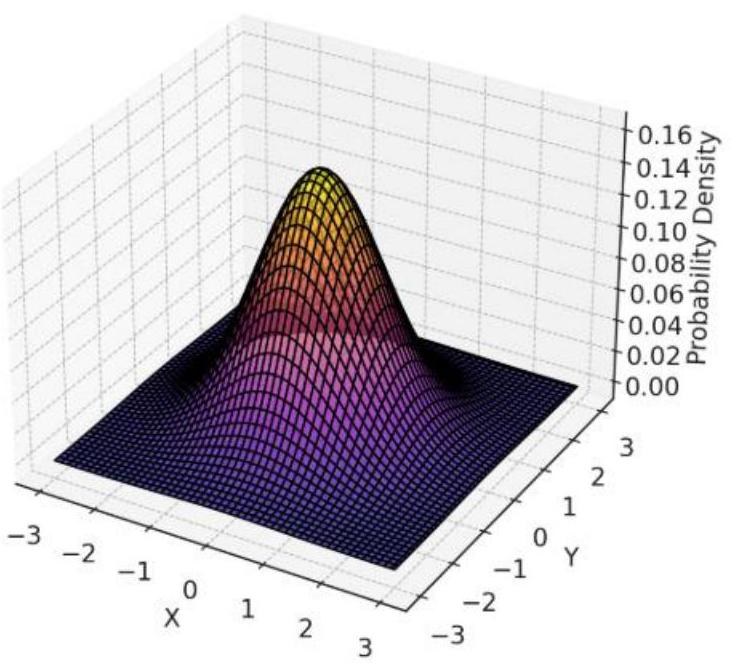
\includegraphics[width=0.6\textwidth]{img-0.jpeg.jpeg}
    \caption{Visualizing the area $P(a_1 < X_1 \le b_1, a_2 < X_2 \le b_2)$ (shaded rectangle) within the context of a 2D distribution. The calculation involves the CDF values at the corners.}
    \label{fig:2d_rect}
\end{figure}

\begin{figure}[htbp]
    \centering
    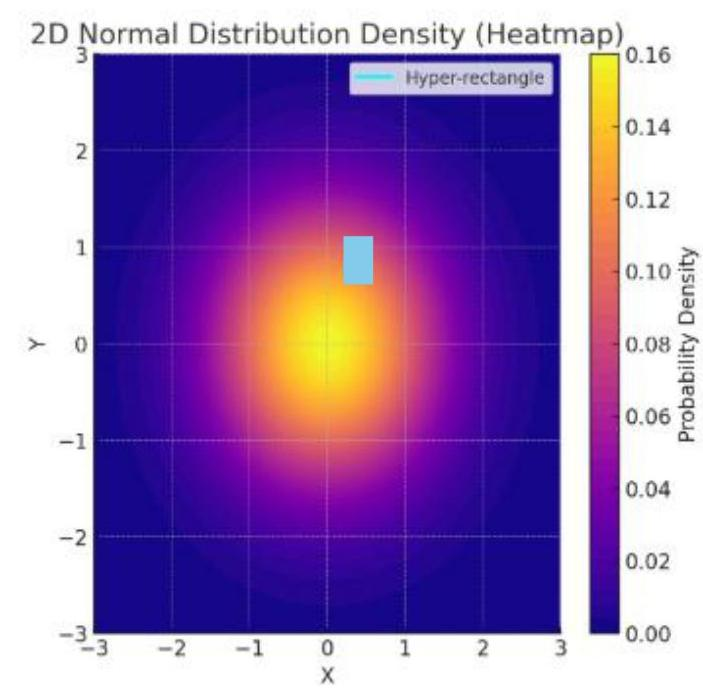
\includegraphics[width=0.6\textwidth]{img-1.jpeg.jpeg}
    \caption{Step 1: $F(b_1, b_2)$ includes the target area plus unwanted regions.}
    \label{fig:2d_step1}
\end{figure}

\begin{figure}[htbp]
    \centering
    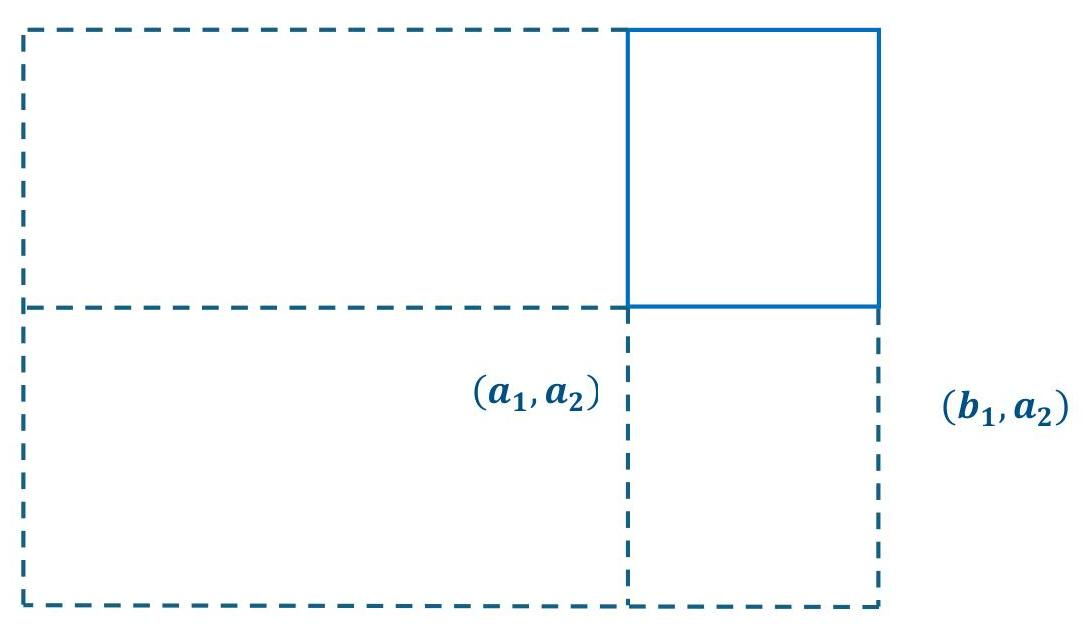
\includegraphics[width=0.6\textwidth]{img-2.jpeg.jpeg}
    \caption{Steps 2, 3, and 4: Subtracting $F(a_1, b_2)$ and $F(b_1, a_2)$, then adding back $F(a_1, a_2)$ isolates the probability of the rectangle $(a_1, b_1] \times (a_2, b_2]$. (Note: The labels $(a_1, b_2)$ and $(b_1, b_2)$ in the image seem misplaced; they should likely refer to the corner coordinates relevant to the inclusion-exclusion steps.)}
    \label{fig:2d_steps234}
\end{figure}

\textbf{Warning:} For $n=3$, you need to imagine this in a 3D room! The calculation involves $2^3=8$ terms corresponding to the corners of the box $(a_1, b_1] \times (a_2, b_2] \times (a_3, b_3]$.

Just as in the 1D case, multivariate distributions can be classified based on the nature of their CDFs.

\subsubsection*{Continuous Random Vectors}

A common and important case is when the joint CDF $F_X(x)$ is absolutely continuous. This means it can be expressed as the integral of a non-negative function called the **joint probability density function (joint PDF)**.

\begin{definition}[Joint PDF]
A random vector $X = (X_1, \dots, X_n)$ is called (absolutely) continuous if there exists a non-negative function $f_X: \R^n \to [0, \infty)$, called the joint probability density function (PDF), such that for all $x = (x_1, \dots, x_n) \in \R^n$:
\[ F_X(x_1, \dots, x_n) = \int_{-\infty}^{x_1} \dots \int_{-\infty}^{x_n} f_X(u_1, \dots, u_n) \, du_n \dots du_1 \]
If $F_X$ is sufficiently smooth, the PDF can be obtained by differentiation:
\begin{equation} \label{eq:pdf_from_cdf}
f_X(x_1, \dots, x_n) = \frac{\partial^n F_X(x_1, \dots, x_n)}{\partial x_1 \partial x_2 \dots \partial x_n}
\end{equation}
provided the derivatives exist.
\end{definition}

\begin{property}[Properties of a Joint PDF]
A function $f: \R^n \to \R$ is a valid joint PDF if and only if:
\begin{enumerate}
    \item $f(x) \ge 0$ for all $x \in \R^n$.
    \item $\int_{\R^n} f(x) \, dx = \int_{-\infty}^{\infty} \dots \int_{-\infty}^{\infty} f(x_1, \dots, x_n) \, dx_n \dots dx_1 = 1$.
\end{enumerate}
\end{property}

For a continuous random vector $X$ with PDF $f_X$, the probability that $X$ falls into a region $A \subseteq \R^n$ is given by the integral of the PDF over that region:
\[ P(X \in A) = \int_{A} f_X(x) \, dx = \iint \dots \int_{A} f_X(x_1, \dots, x_n) \, dx_n \dots dx_1 \]
Note that for continuous random vectors, the probability of $X$ taking any single specific value $x_0$ is zero, i.e., $P(X = x_0) = 0$. This also means $P(X \le x) = P(X < x)$.

\begin{example}[Uniform Distribution on a Hyper-rectangle] \label{ex:uniform_box}
Consider an experiment where we measure the position $(X_1, X_2, X_3)$ of an item moving randomly within a box $[a_1, b_1] \times [a_2, b_2] \times [a_3, b_3]$. If the position is equally likely to be anywhere within the box, the random vector $X = (X_1, X_2, X_3)$ follows a **uniform distribution** on this hyper-rectangle (a box in 3D).
Let $R = [a_1, b_1] \times \dots \times [a_n, b_n]$ be a hyper-rectangle in $\R^n$. The random vector $X$ has a uniform distribution on $R$ if its joint PDF is:
\[ f_X(x_1, \dots, x_n) = \begin{cases}
    \frac{1}{\text{Volume}(R)} & \text{if } (x_1, \dots, x_n) \in R \\
    0 & \text{otherwise}
\end{cases} \]
where $\text{Volume}(R) = (b_1 - a_1)(b_2 - a_2)\dots(b_n - a_n)$.
For the 3D case mentioned ($n=3$), the PDF is $f_X(x_1, x_2, x_3) = 1/((b_1-a_1)(b_2-a_2)(b_3-a_3))$ for $x_i \in [a_i, b_i]$, and 0 otherwise.
\textbf{Application Context:} This type of distribution is relevant, for instance, in robotics where robots might sample locations or orientations uniformly within a 3D workspace for tasks like motion planning, exploration, or coverage.
\end{example}

\subsubsection*{Discrete Random Vectors}

Another important case is when the random vector $X$ can only take values in a finite or countably infinite set $\mathcal{S} \subset \R^n$. Such vectors are called **discrete random vectors**. Their distribution is characterized by a **joint probability mass function (joint PMF)**.

\begin{definition}[Joint PMF]
A random vector $X = (X_1, \dots, X_n)$ is called discrete if it takes values in a countable set $\mathcal{S} = \{x^{(1)}, x^{(2)}, \dots\} \subset \R^n$. Its joint probability mass function (PMF) is the function $p_X: \R^n \to [0, 1]$ defined by:
\[ p_X(x) = P(X = x) \]
Note that $p_X(x) > 0$ only if $x \in \mathcal{S}$, and $p_X(x) = 0$ if $x \notin \mathcal{S}$.
\end{definition}

\begin{property}[Properties of a Joint PMF]
A function $p: \R^n \to \R$ is a valid joint PMF if and only if:
\begin{enumerate}
    \item $p(x) \ge 0$ for all $x \in \R^n$.
    \item $\sum_{x \in \mathcal{S}} p(x) = 1$, where the sum is over the countable support set $\mathcal{S}$.
\end{enumerate}
\end{property}

For a discrete random vector $X$ with PMF $p_X$, the probability that $X$ falls into a region $A \subseteq \R^n$ is given by summing the PMF over the points in the support set $\mathcal{S}$ that are also in $A$:
\[ P(X \in A) = \sum_{x \in A \cap \mathcal{S}} p_X(x) \]
The joint CDF $F_X(x)$ for a discrete random vector is obtained by summing the PMF over all points $u \in \mathcal{S}$ such that $u \le x$ (component-wise):
\[ F_X(x) = \sum_{u \in \mathcal{S}, u \le x} p_X(u) \]
The CDF will be a step function in $n$ dimensions.

\begin{example}[Multinomial Distribution] \label{ex:multinomial}
The **Multinomial distribution** is a multivariate generalization of the Binomial distribution. Consider an experiment with $k$ possible outcomes (categories), where the probability of outcome $i$ is $p_i$, with $p_i \ge 0$ and $\sum_{i=1}^k p_i = 1$. Suppose we perform $n$ independent trials of this experiment. Let $X_i$ be the number of times outcome $i$ occurs in the $n$ trials. The random vector $X = (X_1, X_2, \dots, X_k)$ follows a Multinomial distribution with parameters $n$ and $p = (p_1, \dots, p_k)$.
Note that the components must sum to $n$: $X_1 + X_2 + \dots + X_k = n$. The vector $p = (p_1, \dots, p_k)$ belongs to the $(k-1)$-dimensional **probability simplex** $\Delta^{k-1} = \{ (p_1, \dots, p_k) \in \R^k \mid p_i \ge 0, \sum_{i=1}^k p_i = 1 \}$.
The joint PMF is given by:
\begin{equation} \label{eq:multinomial_pmf}
p_X(x_1, \dots, x_k) = P(X_1=x_1, \dots, X_k=x_k) = \frac{n!}{x_1! x_2! \dots x_k!} p_1^{x_1} p_2^{x_2} \dots p_k^{x_k}
\end{equation}
for non-negative integers $x_i \in \N \cup \{0\}$ such that $\sum_{i=1}^k x_i = n$. The PMF is 0 for any other values $(x_1, \dots, x_k)$.
(When $k=2$, we have $X_1 = x_1$, $X_2 = n-x_1$, $p_1=p$, $p_2=1-p$, and the formula reduces to the Binomial PMF: $\frac{n!}{x_1!(n-x_1)!} p^{x_1} (1-p)^{n-x_1}$).
This is a discrete distribution on $\mathbb{Z}^k$.
\end{example}

\subsubsection*{Mixed and Singular Distributions}

Of course, the relationship between discrete and continuous parts can be much more intricate in $\R^n$ (for $n > 1$) due to the richer geometric structure. In particular, probability mass might be concentrated on lower-dimensional subspaces (lines, surfaces, etc.). Such distributions are neither purely discrete nor absolutely continuous. The following example illustrates this.

\begin{example}[Singular Distribution on a Line] \label{ex:singular_diagonal}
Let $S$ be a continuous 1-dimensional random variable with CDF $F_S(s)$ and PDF $f_S(s)$. Define a 2-dimensional random vector $X$ as $X = (S, S)$. That is, $X_1 = S$ and $X_2 = S$. Let's find the joint CDF of $X=(X_1, X_2)$.
For any $(x_1, x_2) \in \R^2$:
\begin{align*}
F_X(x_1, x_2) &= P(X_1 \le x_1, X_2 \le x_2) \\
&= P(S \le x_1, S \le x_2) \\
&= P(S \le \min(x_1, x_2)) \\
&= F_S(\min(x_1, x_2)) \label{eq:singular_cdf} \tag{2.3}
\end{align*}
Now, let's ask: does this random vector $X$ have a joint PDF $f_X(x_1, x_2)$? If it did, we should be able to obtain it via differentiation as in \eqref{eq:pdf_from_cdf}: $f_X(x_1, x_2) = \frac{\partial^2 F_X(x_1, x_2)}{\partial x_1 \partial x_2}$.
However, consider the region where $x_1 \ne x_2$.
If $x_1 < x_2$, then $\min(x_1, x_2) = x_1$, so $F_X(x_1, x_2) = F_S(x_1)$. Then $\frac{\partial F_X}{\partial x_2} = 0$.
If $x_2 < x_1$, then $\min(x_1, x_2) = x_2$, so $F_X(x_1, x_2) = F_S(x_2)$. Then $\frac{\partial F_X}{\partial x_1} = 0$.
In both cases (i.e., whenever $x_1 \ne x_2$), the second partial derivative $\frac{\partial^2 F_X}{\partial x_1 \partial x_2}$ is 0.
This would imply $f_X(x_1, x_2) = 0$ almost everywhere. But if $f_X$ is zero almost everywhere, its integral over $\R^2$ would be 0, not 1, contradicting the property of a PDF.
What went wrong? The issue is that the probability mass of $X=(S,S)$ is entirely concentrated on the line $x_1 = x_2$ in the $\R^2$ plane. This line has zero area (2D measure). A joint PDF describes density with respect to area; you can't use it to describe mass concentrated on a line. The partial derivatives in \eqref{eq:pdf_from_cdf} do not exist in a meaningful way along the diagonal $x_1 = x_2$.
So, the random vector $X=(S, S)$ is neither discrete (since $S$ is continuous, $X$ can take uncountably many values on the line $x_1=x_2$) nor is it absolutely continuous (as it lacks a joint PDF). It's an example of a **singular distribution** (relative to 2D Lebesgue measure). The probability $P(X_1 = X_2) = P(S=S) = 1$, which is obvious, but this cannot be captured by integrating a PDF $f_X(x_1, x_2)$.
\end{example}

\subsubsection*{Marginal Distributions}

Often, even if we have the joint distribution of $X = (X_1, \dots, X_n)$, we might be interested in the distribution of just one component, say $X_i$, or a subset of components, say $(X_{i_1}, \dots, X_{i_k})$. These are called **marginal distributions**.

We can obtain the marginal CDF of a subset of variables from the joint CDF by letting the arguments corresponding to the *other* variables go to $+\infty$. For instance, the marginal CDF of $X_1$ is:
\[ F_{X_1}(x_1) = P(X_1 \le x_1) = P(X_1 \le x_1, X_2 < \infty, \dots, X_n < \infty) = \lim_{x_2 \to \infty, \dots, x_n \to \infty} F_X(x_1, x_2, \dots, x_n) \]
More generally, the marginal CDF of a sub-vector $X_{\mathcal{I}} = (X_i)_{i \in \mathcal{I}}$ for some index set $\mathcal{I} \subset \{1, \dots, n\}$ is obtained by taking the limit as $x_j \to \infty$ for all $j \notin \mathcal{I}$.

If the random vector $X$ has a joint PDF $f_X(x_1, \dots, x_n)$, then any sub-vector $X_{\mathcal{I}}$ also has a marginal PDF, obtained by integrating the joint PDF over all possible values of the variables *not* in $X_{\mathcal{I}}$. For example, the marginal PDF of $X_1$ is:
\[ f_{X_1}(x_1) = \int_{-\infty}^{\infty} \dots \int_{-\infty}^{\infty} f_X(x_1, x_2, \dots, x_n) \, dx_n \dots dx_2 \]
And the marginal PDF of $(X_1, X_2)$ (if $n \ge 2$) is:
\[ f_{X_1, X_2}(x_1, x_2) = \int_{-\infty}^{\infty} \dots \int_{-\infty}^{\infty} f_X(x_1, x_2, x_3, \dots, x_n) \, dx_n \dots dx_3 \]
We are essentially "integrating out" the variables we are not interested in.

Similarly, if $X$ has a joint PMF $p_X(x_1, \dots, x_n)$ with support $\mathcal{S}$, the marginal PMF of a sub-vector $X_{\mathcal{I}}$ is obtained by summing the joint PMF over all possible values of the variables *not* in $X_{\mathcal{I}}$. For example, the marginal PMF of $X_1$ is:
\[ p_{X_1}(x_1) = \sum_{x_2, \dots, x_n \text{ s.t. } (x_1, x_2, \dots, x_n) \in \mathcal{S}} p_X(x_1, x_2, \dots, x_n) \]
We are "summing out" the unwanted variables.

\begin{remark}
Knowing the marginal distributions is generally *not* enough to determine the joint distribution. The joint distribution contains information about the dependencies between variables, which is lost when looking only at the marginals. We will explore this further when we discuss independence. The following example highlights that different joint distributions can share the same marginals.
\end{remark}

\begin{example}[Same Marginals, Different Joint PDF - Not presented in lecture] \label{ex:fgm}
Consider a pair of continuous random variables $(X, Y)$ with a joint PDF given by:
\[ f_{X,Y}(x,y) = f_X(x) f_Y(y) [1 + \alpha (2F_X(x) - 1)(2F_Y(y) - 1)] \]
where $f_X(x)$ and $f_Y(y)$ are valid 1-dimensional PDFs with corresponding CDFs $F_X(x)$ and $F_Y(y)$, and $\alpha$ is a constant such that $|\alpha| \le 1$.
(This form is related to the Farlie-Gumbel-Morgenstern copula family).

First, let's check if this is a valid PDF. Since $f_X, f_Y \ge 0$, and $0 \le F_X, F_Y \le 1$, the terms $(2F_X(x)-1)$ and $(2F_Y(y)-1)$ range between -1 and +1. Thus, the factor $[1 + \alpha (\dots)(\dots)]$ ranges between $1-|\alpha|$ and $1+|\alpha|$. Since $|\alpha| \le 1$, this factor is non-negative, ensuring $f_{X,Y}(x,y) \ge 0$.

Second, let's check if it integrates to 1:
\begin{align*}
\int_{-\infty}^{\infty} \int_{-\infty}^{\infty} f_{X,Y}(x,y) \, dx \, dy &= \int f_Y(y) \left[ \int f_X(x) [1 + \alpha (2F_X(x) - 1)(2F_Y(y) - 1)] \, dx \right] dy \\
&= \int f_Y(y) \left[ \int f_X(x) dx + \alpha (2F_Y(y) - 1) \int f_X(x) (2F_X(x) - 1) \, dx \right] dy
\end{align*}
We know $\int f_X(x) dx = 1$. Let's evaluate the other integral. Let $u = F_X(x)$, then $du = f_X(x) dx$. As $x$ goes from $-\infty$ to $\infty$, $u$ goes from 0 to 1.
\[ \int_{-\infty}^{\infty} f_X(x) (2F_X(x) - 1) \, dx = \int_0^1 (2u - 1) \, du = [u^2 - u]_0^1 = (1-1) - (0-0) = 0 \]
So, the inner integral simplifies to $1 + \alpha (2F_Y(y) - 1) \cdot 0 = 1$.
Therefore,
\[ \int_{-\infty}^{\infty} \int_{-\infty}^{\infty} f_{X,Y}(x,y) \, dx \, dy = \int_{-\infty}^{\infty} f_Y(y) [1] \, dy = 1 \]
So, $f_{X,Y}(x,y)$ is indeed a valid joint PDF for any $|\alpha| \le 1$.

Now, let's find the marginal PDFs.
Marginal PDF for X:
\begin{align*}
f_{X}(x) &= \int_{-\infty}^{\infty} f_{X,Y}(x,y) \, dy \\
&= \int f_X(x) f_Y(y) [1 + \alpha (2F_X(x) - 1)(2F_Y(y) - 1)] \, dy \\
&= f_X(x) \int f_Y(y) dy + f_X(x) \alpha (2F_X(x) - 1) \int f_Y(y) (2F_Y(y) - 1) \, dy
\end{align*}
Again, $\int f_Y(y) dy = 1$, and by the same argument as before, $\int f_Y(y) (2F_Y(y) - 1) dy = 0$.
So, $f_X(x) = f_X(x) \cdot 1 + f_X(x) \alpha (2F_X(x) - 1) \cdot 0 = f_X(x)$.
Similarly, integrating out $x$, we find the marginal PDF for Y is $f_Y(y)$.

The crucial point here is that the marginal PDFs are $f_X(x)$ and $f_Y(y)$, *regardless* of the value of $\alpha$ (as long as $|\alpha| \le 1$). This means we can have a whole family of different joint distributions (corresponding to different $\alpha$'s, which control the dependency structure) that all share the exact same marginal distributions. This clearly demonstrates that marginals do not determine the joint distribution.
\end{example}

\begin{remark}
You will encounter various examples of multivariate distributions and their marginals in the exercises.
\end{remark}

\subsection{Expectation}

Just as we compute the expected value (or mean) of a scalar random variable, we can compute the expected value of a random vector. The idea extends naturally.

Let $X = (X_1, \dots, X_n)$ be a random vector. If $h$ is a function mapping from $\R^n$ to $\R^m$, say $h: \R^n \to \R^m$, then $Y = h(X)$ is also a random vector (taking values in $\R^m$). We can compute its expectation, $\E[Y] = \E[h(X)]$.

\begin{definition}[Expectation of a Function of a Random Vector]
Let $X$ be a random vector in $\R^n$, and let $h: \R^n \to \R^m$ be a function.
\begin{itemize}
    \item If $X$ is continuous with joint PDF $f_X(x)$, then the expectation of $Y = h(X)$ is defined as:
    \[ \E[Y] = \E[h(X)] = \int_{\R^n} h(x) f_X(x) \, dx \]
    This is a vector in $\R^m$, where the integral is performed component-wise for the vector function $h(x) = (h_1(x), \dots, h_m(x))$.
    \item If $X$ is discrete with joint PMF $p_X(x)$ and support $\mathcal{S}$, then the expectation is:
    \[ \E[Y] = \E[h(X)] = \sum_{x \in \mathcal{S}} h(x) p_X(x) \]
    This is also a vector in $\R^m$, computed component-wise.
\end{itemize}
The expectation is defined only if each component of the integral (or sum) converges absolutely. That is, for the continuous case, $\int_{\R^n} |h_i(x)| f_X(x) dx < \infty$ for all $i=1, \dots, m$. Similarly for the discrete case.
\end{definition}

A particularly important special case is the expectation of the random vector $X$ itself. This corresponds to $h(x) = x$ (so $m=n$).

\begin{definition}[Expectation of a Random Vector]
The expectation (or mean vector) of a random vector $X = (X_1, \dots, X_n)$ is the vector of the expectations of its components:
\[ \E[X] = \begin{pmatrix} \E[X_1] \\ \E[X_2] \\ \vdots \\ \E[X_n] \end{pmatrix} \]
provided each $\E[X_i]$ exists.
\end{definition}

Many properties of expectation from the 1D case extend naturally to the multivariate setting, respecting the rules of vector and matrix algebra.

\begin{property}[Properties of Expectation for Random Vectors]
Let $X$ and $Y$ be random vectors (of appropriate dimensions) and let $A$ and $B$ be constant matrices (or vectors, as special cases) of appropriate dimensions.
\begin{enumerate}
    \item \textbf{Linearity:}
    \begin{equation} \label{eq:linearity_E}
    \E[AX + BY] = A\E[X] + B\E[Y] \tag{2.4}
    \end{equation}
    This holds provided $\E[X]$ and $\E[Y]$ exist.
\end{enumerate}
\end{property}

Beyond the mean vector, we need ways to describe the variability and dependencies within the random vector. This leads to the concept of the covariance matrix.

\begin{definition}[Covariance Matrix]
Let $X$ be an $n$-dimensional random vector with mean vector $\mu_X = \E[X]$, and let $Y$ be an $m$-dimensional random vector with mean vector $\mu_Y = \E[Y]$.
\begin{itemize}
    \item The **cross-covariance matrix** between $X$ and $Y$ is the $n \times m$ matrix defined as:
    \begin{align*} \Cov(X, Y) &= \E[(X - \mu_X)(Y - \mu_Y)^T] \\ &= \E[XY^T] - \mu_X \mu_Y^T \end{align*}
    The $(i, j)$-th element of this matrix is $\Cov(X_i, Y_j) = \E[(X_i - \mu_{X_i})(Y_j - \mu_{Y_j})]$.
    \item The **covariance matrix** (or variance-covariance matrix) of the random vector $X$ is the $n \times n$ matrix obtained by setting $Y=X$:
    \begin{align*} \Cov(X) = \Cov(X, X) &= \E[(X - \mu_X)(X - \mu_X)^T] \\ &= \E[XX^T] - \mu_X \mu_X^T \end{align*}
\end{itemize}
These expectations are defined if the relevant second moments exist.
\end{definition}

Let's look closer at the covariance matrix $\Cov(X)$ for $X = (X_1, \dots, X_n)^T$:
\[ \Cov(X) = \begin{pmatrix}
\E[(X_1-\mu_1)(X_1-\mu_1)] & \E[(X_1-\mu_1)(X_2-\mu_2)] & \dots & \E[(X_1-\mu_1)(X_n-\mu_n)] \\
\E[(X_2-\mu_1)(X_1-\mu_1)] & \E[(X_2-\mu_2)(X_2-\mu_2)] & \dots & \E[(X_2-\mu_2)(X_n-\mu_n)] \\
\vdots & \vdots & \ddots & \vdots \\
\E[(X_n-\mu_1)(X_1-\mu_1)] & \E[(X_n-\mu_2)(X_2-\mu_2)] & \dots & \E[(X_n-\mu_n)(X_n-\mu_n)]
\end{pmatrix} \]
\[ = \begin{pmatrix}
\Var(X_1) & \Cov(X_1, X_2) & \dots & \Cov(X_1, X_n) \\
\Cov(X_2, X_1) & \Var(X_2) & \dots & \Cov(X_2, X_n) \\
\vdots & \vdots & \ddots & \vdots \\
\Cov(X_n, X_1) & \Cov(X_n, X_2) & \dots & \Var(X_n)
\end{pmatrix} \]
The diagonal elements are the variances of the individual components $X_i$. The off-diagonal element $(i, j)$ is the covariance between $X_i$ and $X_j$. Since $\Cov(X_i, X_j) = \Cov(X_j, X_i)$, the covariance matrix is always **symmetric**.

\begin{property}[Properties of the Covariance Matrix]
Let $X$ be an $n$-dimensional random vector with covariance matrix $\Cov(X)$.
\begin{enumerate}
    \item $\Cov(X)$ is symmetric, i.e., $\Cov(X)^T = \Cov(X)$.
    \item $\Cov(X)$ is **positive semi-definite**. This means that for any constant vector $v \in \R^n$, the quadratic form $v^T \Cov(X) v \ge 0$.
    \item If $A$ is a constant $m \times n$ matrix, then the covariance matrix of the transformed vector $Y = AX$ is $\Cov(Y) = A \Cov(X) A^T$.
\end{enumerate}
\end{property}

\begin{proof}[Proof of Positive Semi-Definiteness]
Let $v \in \R^n$ be any constant vector. Consider the scalar random variable $Z = v^T(X - \E[X])$. The variance of $Z$ is:
\begin{align*}
\Var(Z) &= \E[(Z - \E[Z])^2] \\
&= \E[(v^T(X - \E[X]) - \E[v^T(X - \E[X])])^2] \\
&= \E[(v^T(X - \E[X]) - v^T\E[X - \E[X]])^2] \quad (\text{linearity of } E) \\
&= \E[(v^T(X - \E[X]) - v^T(0))^2] \\
&= \E[(v^T(X - \E[X]))^2] \\
&= \E[(v^T(X - \E[X])) (v^T(X - \E[X]))^T] \quad (\text{since } Z \text{ is scalar, } Z = Z^T) \\
&= \E[v^T(X - \E[X]) (X - \E[X])^T v] \\
&= v^T \E[(X - \E[X]) (X - \E[X])^T] v \quad (\text{taking constants } v, v^T \text{ out of } E) \\
&= v^T \Cov(X) v
\end{align*}
Since variance is always non-negative, $\Var(Z) \ge 0$. Therefore, $v^T \Cov(X) v \ge 0$ for all $v \in \R^n$, which proves that $\Cov(X)$ is positive semi-definite.
\end{proof}

The covariance matrix $\Cov(X)$ is a fundamental tool that summarizes the second-order structure of the random vector $X$. It captures not only the spread of each component (through the variances on the diagonal) but also the pairwise linear dependencies between components (through the covariances off the diagonal). We will delve deeper into the interpretation and use of the covariance matrix later, particularly when discussing topics like the multivariate normal distribution and principal component analysis.

\subsection{Moment Generating Functions}

(At this stage, due to time constraints, we will not cover this in the lecture – it will be sent later as reading material.)

\end{document}